\begin{document}
\newpage
\subsection{Meranie a analýza nameraných dát}
\begin{figure}[h!]
    \centering
    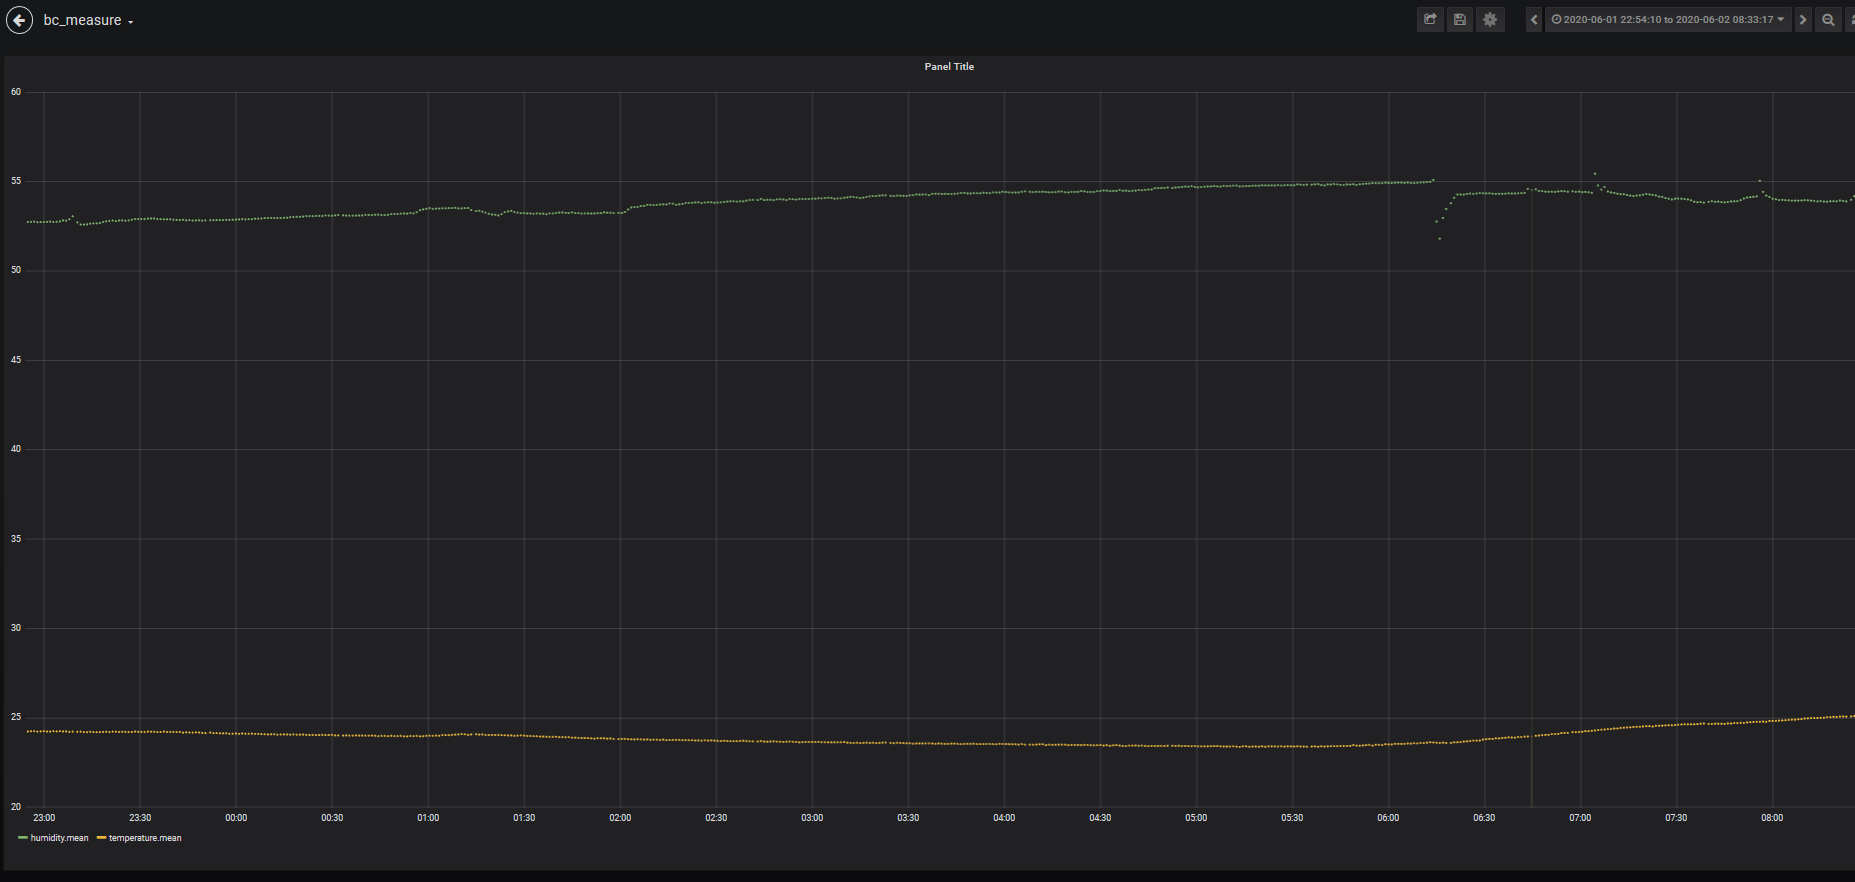
\includegraphics[width = 0.65\textwidth]{images/measurement.png}
    \caption{Namerané dáta z vývojovej dosky Heltec LoRaWAN32}
    \label{fig:measurement}
\end{figure}
\begin{wrapfigure}{r}[-12mm]{0.35\textwidth}
    \centering
    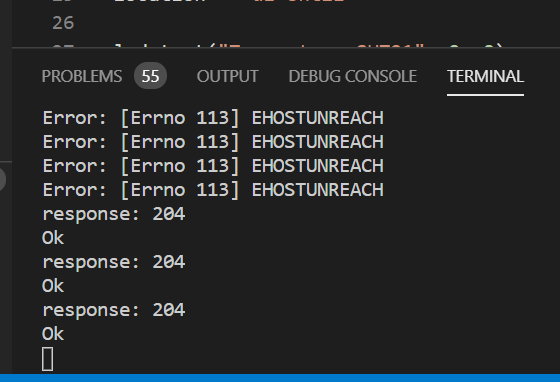
\includegraphics[width = 0.34\textwidth]{images/fail.png}
    \caption{Vypísanie chybovej hlášky pri nedostupnosti služby}
    \label{fig:fail}
\end{wrapfigure}
Namerané dáta z vývojovej dosky dokážem ukladať do Cloudovej služby pomocou naštartovaného kontajnera s prostredím pre ukladanie a vizualizáciu dát. V Grafane je možné odosielať rôzne správy pri prekročení kritických hodnôt. Pomocou takejto metódy nemám starosti o serverovú infraštruktúru.
\vfill
\clearpage
\end{document}
